\chapter{Concept \& Design}
\label{cha:cod}

\section{Application Architecture}
\label{section:software_architecture}

BASED ON ZERO_TRUST PRINCIPLES NENNEN?!?! DAPP NENNEN?, SERVICE ORIENTED ARCHITECTURE, MICROSERVICES

This section defines the main architectural components of the proposed decentralized, blockchain-based data marketplace. Although it can be run by any central party or deployed on any cloud infrastructure, it is intended to be deployed on the operator's own local on-premises infrastructure. This eliminates trust in central servers and ensures great control over the data, as it never leaves the operator's premises. It also provides excellent flexibility, as each operator can scale its own infrastructure independently, deploying only the components he or she needs. The complete software stack, as shown in figure \ref{fig:arch}, consists of a full Ethereum node, a blockchain indexer, an IPFS node, a compute microservice, a crypto microservice, a message queue, and an API gateway.

%This section defines the main software components of our decentralized blockchain-based data marketplace. Although it can be run by any central party or deployed to any cloud infrastructure, it is intended to be deployed on the operator's own local on-premises infrastructure. This eliminates the trust in central servers and ensures great control over data as it never has to leave the operator's boundaries. Furthermore, it ensures high flexibility since every operator can independently scale their own infrastructure and only needs to deploy the necessary components according to their needs. The full software stack as depicted in figure \ref{fig:arch} is composed of an Ethereum full node, a blockchain indexer, an IPFS node, a compute microservice, a crypto microservice, a message queue, and an API gateway. The following sections describe those components in more detail.

%Accordingly, our main objectives were to make the platform as available, scalable, and decentralized as possible, while maintaining the highest level of security. The former is achieved by forcing each user of Taia-X to deploy the entire platform on their own local infrastructure. This eliminates the need for a centralized server. The latter aspect is realized by keeping the entry points to our platform as minimal as possible and secured by an access control mechanism. Our platform consists of a Tezos full node, blockchain indexers, a frontend, a backend, and a node, as shown in Figure 5.1. A more detailed diagram of the final architecture, including the technologies, can be found in Figure 2. The following sections describe the components in more detail.
        
\begin{figure}[!htb]
    \centering
    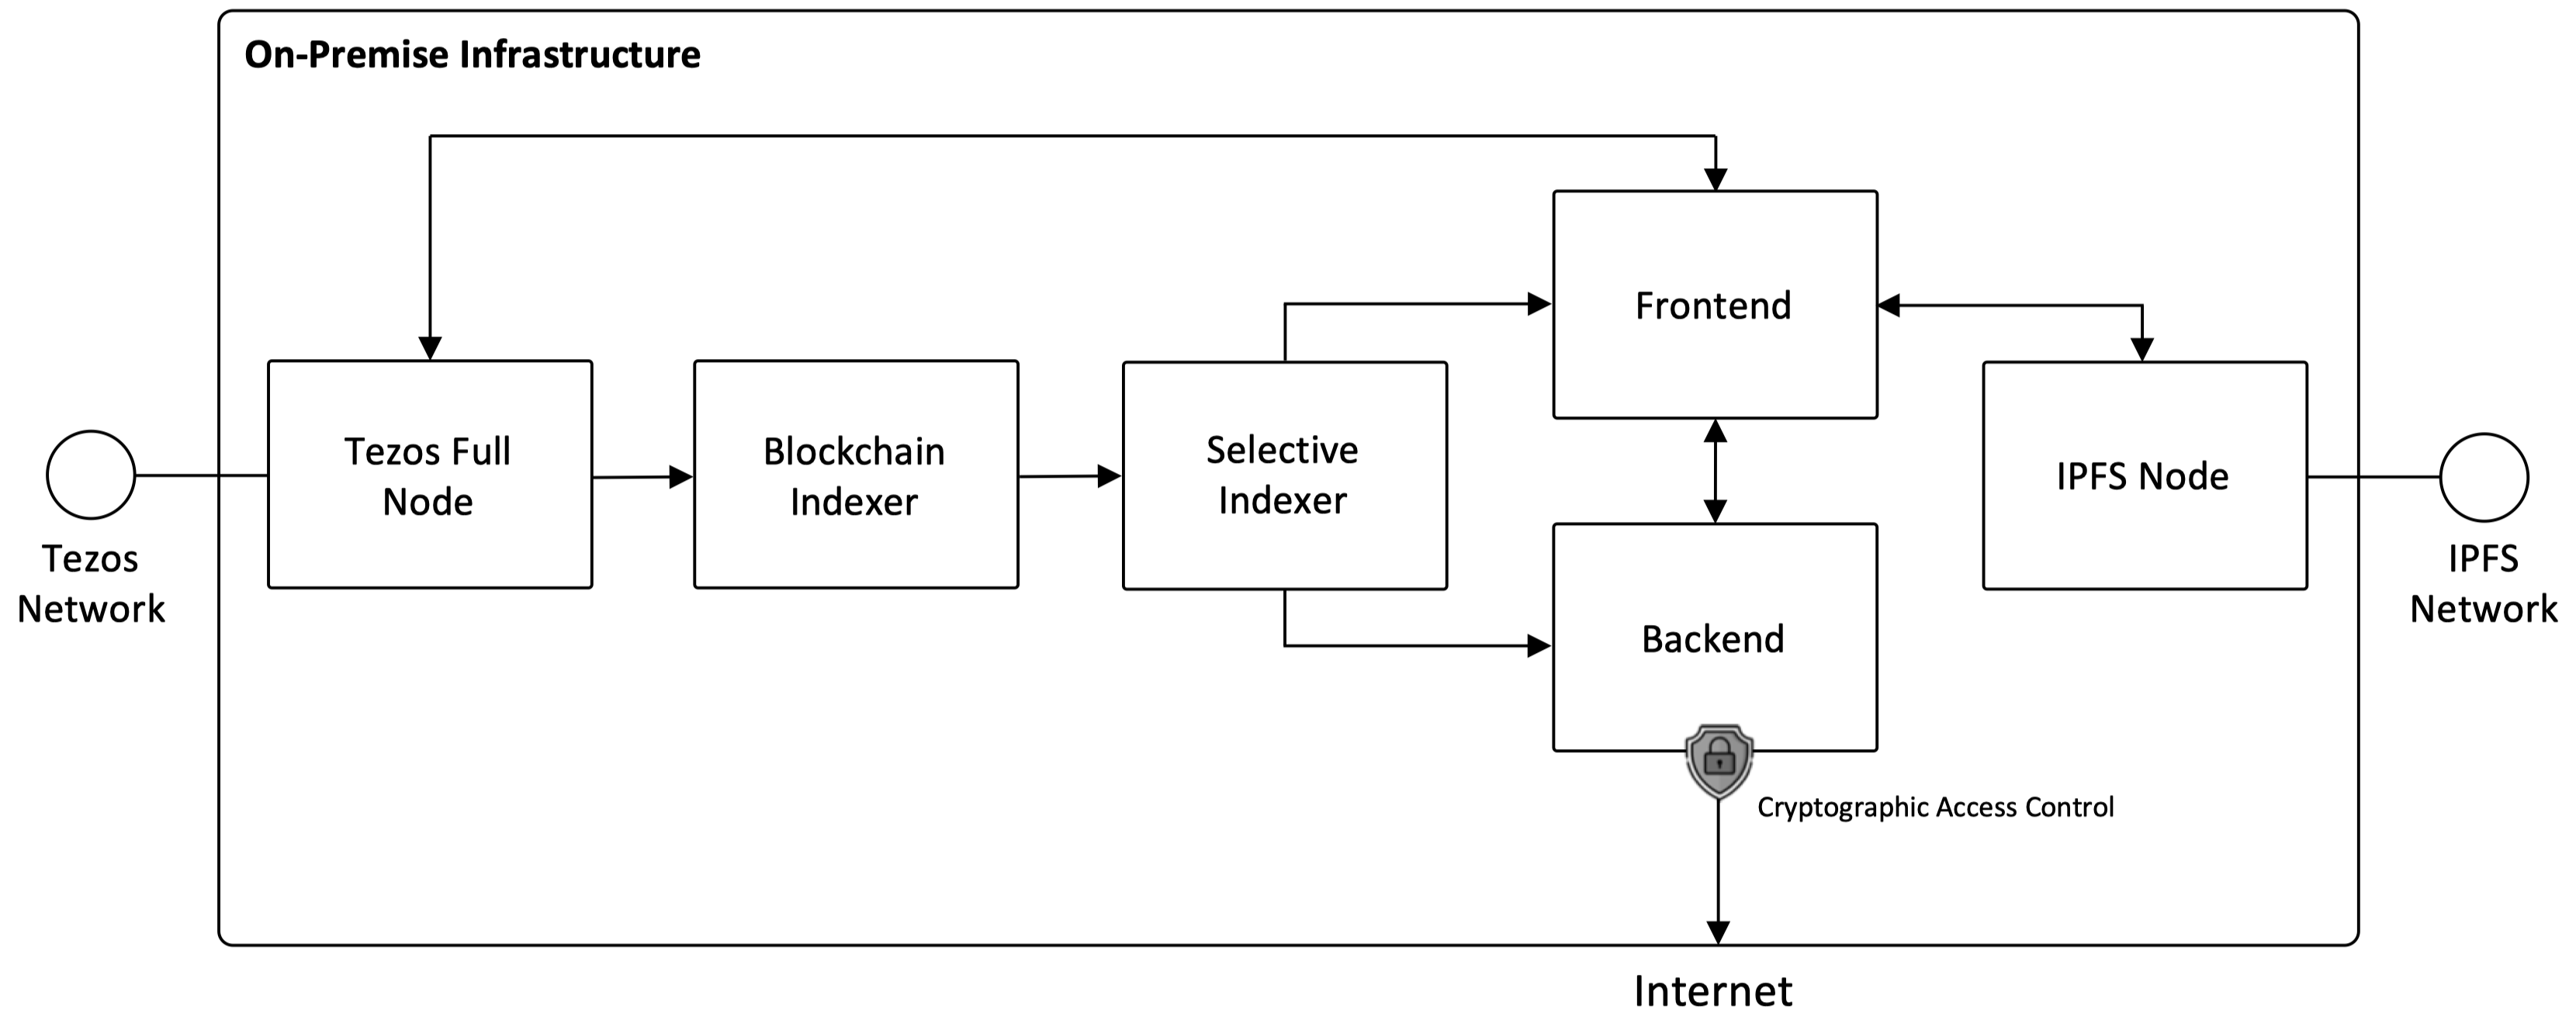
\includegraphics[width=14cm]{images/arch.png}
    \caption[High Level Software Architecture Diagram of Taia-X]{High Level Software Architecture Diagram of Taia-X including the Data Flow}
    \label{fig:arch}
\end{figure}

\subsection{Ethereum Full Node}

An Ethereum full node is a piece of hardware, most often a consumer-grade computer, that runs the client software to download an entire copy of the Ethereum blockchain. It is connected to other nodes, forming a geographically diverse decentralized peer-to-peer (P2P) network, and is responsible for verifying the validity of all blocks and transactions. To interact with the blockchain, users need to sign transactions with their wallet and send them to an RPC node. However, most wallets point to a public RPC node, such as Infura\footnote{https://www.infura.io/} or Alchemy\footnote{https://www.alchemy.com/}, which is considered a centralized trusted third party and often involves additional usage costs. This inevitably leads to a number of problems.

First, any transaction sent to a public RPC endpoint poses a privacy and security risk, as they can potentially leak balances and other personal information by linking an IP address to an Ethereum account address. In addition, public RPC endpoints could even reject or manipulate transactions, making it impossible to interact with the blockchain. Furthermore, centralized solutions provide an attack surface for malicious actors, disrupting the network and leading to a single point of failure.

The implementation of own Ethereum full nodes aligns well with zero trust principles and allows to interact with the blockchain in a trustless, privacy-preserving, and secure manner. It eliminates censorship and single point of failure while making the network more reliable, robust, and geographically diverse. Likewise, it is relatively easy and affordable to deploy an Ethereum full node. Although not recommended, it could even run on a lightweight single-board computer (SBC) such as a Raspberry Pi with enough external storage.

%A blockchain full node typically stores an entire copy of the distributed ledger and validates transactions and blocks. To be able to interact with the blockchain, decentralized applications usually leverage RPC calls to send transactions to - and receive data from a node. However, most decentralized applications connect via community-run\footnote{https://tezostaquito.io/docs/rpc\_nodes/} nodes, which are publicly available. Unfortunately, these nodes can be considered as trustful central entities. A user essentially trusts these nodes not to modify their requests, as well as not to censor operations. Additionally, community-run nodes can be unavailable in case of network partitioning. Hence, every deployment of Taia-X includes its own Tezos Full Node.
            
%Firstly, it helps the network to grow and implicitly makes it more secure by following the network's protocol. Secondly, users of Taia-X don't have to trust public servers to handle transactions to - and queries from the blockchain correctly. Thirdly, it keeps the user's privacy safe, because transactions are not broadcasted to a central server that can leak the user's address. Lastly, it is not complicated and very affordable to deploy a Tezos Full Node.
            
\subsection{Blockchain Indexer}
\label{subsec:indexer}
            
%Every decentralized application relies heavily on information from the blockchain. Due to the natural transparency of public permissionless blockchains, it is possible to inspect every information from the decentralized ledger. However, the ledger is a time-ordered append-only data structure, which makes it highly inefficient to filter, search, paginate, aggregate, or in general query it. Unfortunately, this should be the bare minimum functionality of every marketplace, to easily find items of interest. Filtering is for example necessary in the user profile of Taia-X, to view collected and created tokens of specific Tezos account addresses. In a typical query, the application would try to find this information across many blocks by traversing the ledger and most probably visit a majority of irrelevant blocks. This is highly inefficient and time-consuming, which is critical in times, where users are used to fast response times in a Web 2.0 space.
            
%We solve this problem, by implementing two Blockchain Indexers in the architecture of Taia-X. Blockchain Indexers typically provide a protocol, to extract raw data from a blockchain node, process the data and store it into a relational database, as soon as a new block is written to the ledger. Additionally, Blockchain Indexers expose an \acrshort{api}, to provide high efficient and fast access to blockchain data with filtering, searching, paginating and aggregating capabilities. This doesn't only have a huge impact on the user experience, but also the developer experience, allowing to conduct queries more easily, with typical API operations or SQL queries, they are already used to.

%However, the majority of decentralized applications leverage publicly available Blockchain Indexers from a centralized server. This makes it a single point of failure in case of network partitioning, an attack vector for fraudulent users, and a less scalable and less performant service in case of high traffic. With Taia-X, every user is responsible for operating their own Blockchain Indexers, which are connected to their own Blockchain Full Node. This doesn't only eliminate all aforementioned aspects, but also eliminates trusting a public centralized service, by reading every information from their own nodes.
            
%The first Blockchain Indexer we introduce is TzKT\footnote{https://github.com/baking-bad/tzkt}. It is directly connected to the Tezos Full Node and reads, processes and stores raw data from \emph{every} newly created block. TzKT serves as the input for the second \emph{selective} Blockchain Indexer, created with DipDup\footnote{https://github.com/dipdup-net/dipdup-py}. This indexer only indexes information of specific smart contracts, which is the marketplace smart contract of Taia-X in our case. We primarily use it to provide Token Metadata, historic data, as well as information regarding accounts, sells and purchases, by exposing an API to achieve near real-time queries from the UI of Taia-X. The selective indexer records information from every newly created block exactly to our needs. This means, we can model our own database and are able to update specific database records, if the state changes over time. Next to that, it allows us to query off-chain token metadata from IPFS and save it directly into the database record of the token. All in all, our Blockchain Indexers result into highly efficient and fast queries from the frontend.

\subsection{Decentralized Application}

A \acrfull{dapp} is an application, that relies on decentralized networks, such as a blockchain, to execute backend application logic and to persist data. In this thesis, the \acrshort{dapp} consists of a frontend user interface that is connected to smart contracts on the Ethereum blockchain, more specifically the \acrshort{evm}. All smart contracts are responsible for executing the protocols in the marketplace in a trustless and censorship-resistant manner with full data integrity, as data stored on the blockchain is immutable. However, it only stores a minimum necessary amount of data to avoid blockchain bloating. Larger amounts of data are stored on other immutable decentralized storages such as IPFS, as described in section \ref{subsec:ipfs}, while leaving a related pointer on the blockchain according to the Content-Addressable Storage Pattern \cite{eberhardtBlockchainInsightsOffChaining2017}

The user interface is the main component for users to interact with the marketplace, i.e. creating computation algorithms, offering computations on private datasets, browsing and filtering the marketplace for interesting offerings as well as making purchases. It is responsible for providing a holistic seamless user experience, however, this is harder to engineer compared to traditional user interfaces, as it introduces a steep learning curve for end-users to understand wallets, transactions, or gas fees among others. In the real world, it is often seen that the frontend part of a \acrshort{dapp} is hosted on centralized cloud servers. However, to be fully decentralized, \acrshort{dapp}s can also be hosted on decentralized \acrshort{p2p} networks such as IPFS, but, the initial loading time could be negatively affected, resulting in a poor user experience. In the proposed marketplace, it is not necessary to host the frontend on IPFS, as each operator hosts its own version of the frontend and doesn't need to trust any centralized servers. %It is even possible to customize the appearance of each user interface.

%Unlike most other blockchain-based marketplaces, our frontend is not hosted on a public centralized server, but deployed on-premise with the rest of Taia-X. It is also imaginable to deploy the frontend on IPFS to keep it decentralized, but the initial loading time with IPFS is mostly too high, resulting into bad user experience and the rejection of Taia-X. For communication, the frontend implements 4 client interfaces to interact with the Blockchain Indexer, the Backend, the IPFS Node and the Wallet.
            
%Since Taia-X is an open source project under the MIT license, it is possible for everyone to modify, add and remove functionality and UI components from the frontend to build a custom version of the UI. However, it is still necessary to adhere to the protocols for communication. The current implementation therefore provides only the basic functionality according to our requirements.
            
\subsection{IPFS Node}
\label{subsec:ipfs}

Storing large amounts of data on the blockchain is very expensive and limited due to block size and gas limitations. For this reason, the proposed marketplace requires a large number of files to be stored on \emph{off-chain} storage. Typical off-chain storage services such as Amazon AWS S3\footnote{https://aws.amazon.com/de/s3/}, Azure Blob Storage\footnote{https://azure.microsoft.com/en-in/services/storage/blobs/} and Google Cloud Storage\footnote{https://cloud.google.com/storage} are easy to use, but they have some significant drawbacks. A cloud storage service is a trusted central third-party system that can be very expensive, vulnerable to cyber-attacks, and unavailable in the event of network partitioning. It also poses a vendor lock-in, making it difficult and costly to switch. Likewise, data stored on cloud storage is not immutable.

The \acrfull{ipfs} is a decentralized peer-to-peer hypermedia protocol for storing and accessing content-addressable files in a distributed file system. An \acrshort{ipfs} node can expose an API to write chunks to the node, and a gateway to read files from the node. While it is possible to leverage public \acrshort{ipfs} nodes, they can represent a single point of failure, just like any cloud storage service. For this reason, each deployment of the proposed marketplace includes an \acrshort{ipfs} node connected to the public \acrshort{ipfs} network. This not only strengthens the network and makes it more geographically diverse, but also replicates and caches files on other nodes, resulting in highly available data. In the proposed marketplace, token metadata, computation algorithms, and evidence key pairs are stored on the \acrshort{ipfs} node and addressable by a \acrfull{cid} that is stored on the blockchain. A \acrshort{cid} is an absolute pointer to the content, similar to a hash of a file, making the content behind the \acrshort{cid} immutable and unique.

%The InterPlanetary File System is a decentralized peer-to-peer hypermedia protocol for storing and accessing files, websites, applications, and data. While it is possible to use some public IPFS nodes for reading from - and writing to the network, it introduces availability and trust problems, such as Cloud Storage Services. For this reason, every deployment of Taia-X includes its own IPFS node. The idea goes hand in hand with running a Blockchain Full Node with each deployment. It is a trustless and highly available node, which helps the network to grow with cheap operating costs. Providers essentially use their local IPFS node to upload token metadata and preview files for each dataset. When other users explore the marketplace of Taia-X and query token metadata, their IPFS node caches the files, making it more and more available and distributed across the planet. This makes it very unlikely that token metadata and preview files ever get lost.
            
\subsection{Compute Service}
\label{subsec:compute}
        
The original idea was to store all datasets on IPFS. However, IPFS is a public peer-to-peer network with no access control, where every Taia-X consumer could access datasets without a purchase. Hence, no data provider would ever adopt Taia-X. To overcome this problem, it is possible to publish only encrypted datasets in IPFS. Nonetheless, data providers would still have no chance to revoke permissions to access datasets and no chance to remove data from the network. Once it is propagated through the IPFS network, it is nearly impossible to remove.
            
With Taia-X, every provider stores their datasets on their own backend component on the file system. This gives data providers full control over their assets. For this reason, the backend exposes an API to upload datasets, which is only accessible from the on-premise internal network. This prevents malicious actors to upload arbitrary and harmful data on the provider's file system from an external network. Additionally, the backend exposes a publicly available download API, to download purchased datasets as a consumer. Since this API endpoint is publicly exposed, it is secured by a cryptographic access control mechanism, which is described in section \ref{subsec:access_control_backend}.

\subsection{Message Queue}
\label{subsec:mq}

\subsection{API Gateway}
\label{subsec:api_gw}

In the proposed marketplace, raw datasets never leave the seller's boundaries to protect PII and confidential data. Instead, buyers can only receive computational results. This data exchange must take place through a secure public channel, i.e. the API gateway. Unlike all other components, the API gateway sits on the public subnet to be accessible by any other marketplace participant. It is the single entry point to the seller's infrastructure, acting as a reverse proxy to route incoming requests to the appropriate microservices on the private subnet. In the proposed marketplace, the API gateway has routes to the compute service, the crypto service, and the blockchain indexer. In addition to routing, it also performs request rate limiting and authorization decisions in a dedicated sidecar container close to the API gateway to avoid latency-intensive network calls

\subsection{Crypto Service}
\label{subsec:crypto}

\section{Smart Contract}
\label{section:smart contract}

\section{Exchange Flow}
\label{section:exchange}

\section{Order Lifecycle}
\label{section:lifecycle}

\section{Stakeholders}
\label{section:stakeholders}

\section{Data Sources}
\label{section:datasource}

%This thesis presents the implementation of a practical real world data marketplace for verifiable statistical computations on private datasets. It addresses \emph{Privacy}, \emph{Fairness} and \emph{Regulation} problems of blockchain-based data trading platforms, while the focus is on \emph{Privacy}. \emph{Furthermore, I only focus on static tabular datasets with very infrequent changes. Hence, I do \textbf{not} focus on real-time streaming data and training of machine-learning models}. My proposed implementation implicitly targets the \emph{Data Transfer} and \emph{Payment} process as well as \emph{IAM} -- some of the fundamental functional requirements, as already depicted in Figure \ref{fig:components}. Specifically, I construct a secure blockchain-based data trading ecosystem, using Blockchain as a medium to (i.) prevent single-point of failure; (ii.) define data usage policies; (iii.) create a transparent, non-repudiable and tamper-proof log of transactions; and (iv.) enforce a fair data exchange protocol. However, the \emph{focus} of this thesis is rather on creating a generic mechanism to make a variety of computations on arbitrary private datasets verifiable, and Blockchain is a necessary part of the puzzle. This thesis uses Verifiable Off-chain Computation (VOC) to address this problem \cite{eberhardtOffchainingModelsApproaches2018,eberhardtBlockchainInsightsOffChaining2017}.

%VOC is a derivative of Verifiable Computation and aims to secure the integrity of computations performed by untrusted parties off the Blockchain. The result of the computation is then published to the Blockchain and verified on-chain with a cryptographic proof, attesting its correctness. Off-loading the computation has multiple benefits -- (i.) it increases the scalability by avoiding complex redundant computations on each node; (ii.) it reduces on-chain transaction costs by significantly lowering the size of transactions; and (iii.) it improves privacy by hiding PII and confidential data from the public ledger. \cite{eberhardtOffchainingModelsApproaches2018,eberhardtZoKratesScalablePrivacyPreserving2018a,simunicVerifiableComputingApplications2021,xuSlimChainScalingBlockchain} 

%According to \cite{eberhardtOffchainingModelsApproaches2018}, a reasonable VC scheme for off-chain computations needs to fulfill the following requirements: (i.) non-interactivity; (ii.) cheap verification; (iii.) weak security assumptions; and (iv.) zero-knowledge. ZkSNARKs, ZkSTARKs and Bulletproofs provide a valid approach to the aforementioned requirements. ZkSNARKs are a type of Zero-knowledge proof (ZKP) that are \emph{non-interactive} and \emph{succinct}. \emph{Non-interactivity} defines the possibility to convince a verifier of a particular statement with only \emph{one} message \cite{eberhardtOffchainingModelsApproaches2018,eberhardtZoKratesScalablePrivacyPreserving2018a,simunicVerifiableComputingApplications2021}. \emph{Succinct} defines a proof that is small in size, compared to ZkSTARKs and Bulletproofs, and can be verified cheaply and quickly, typically within a few milliseconds \cite{simunicVerifiableComputingApplications2021}. This thesis uses a ZKP with ZkSNARKs for verifiable computations on private datasets.

%The proposed blockchain-based data trading platform is designed for two party relationships between a buyer \emph{B} and seller \emph{S}. The current high-level protocol for a trade between \emph{B} and \emph{S} on the proposed platform is described by the following exemplary use case and shown in the subsequent Figure \ref{fig:usecase}, without technical details.

\begin{figure}[!htb]
    \centering
    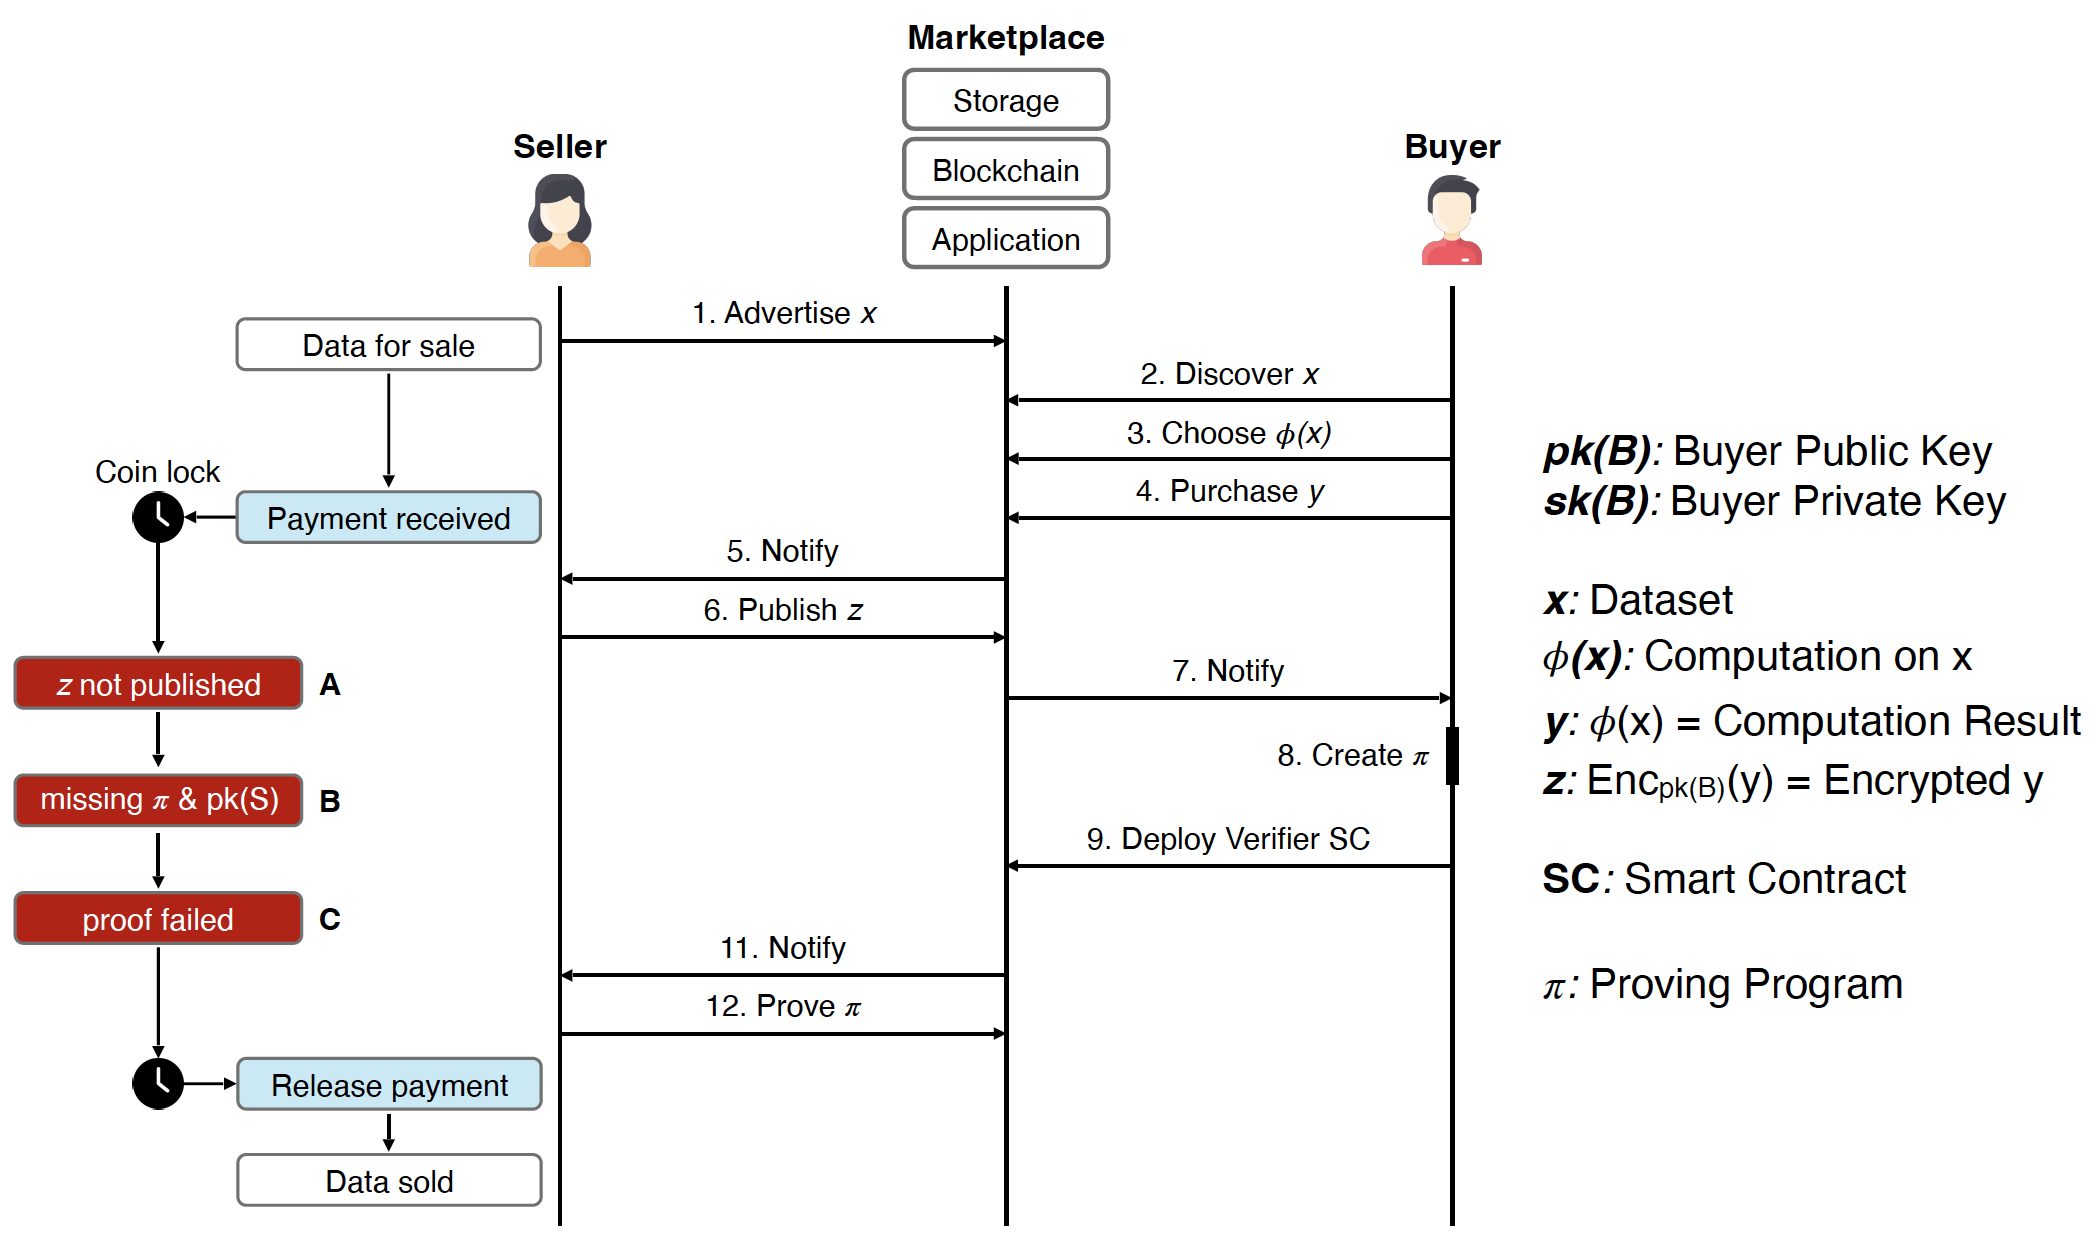
\includegraphics[width=14cm]{images/protocol.png}
    \caption{Proposed protocol for a blockchain-based data trading platform with Compute-to-Data and Verifiable Off-chain Computation for verifiable statistical queries on private datasets. The marketplace between a buyer \emph{B} and seller \emph{S} is highly abstracted into storage, Blockchain and application components, which are necessary for the entire data marketplace ecosystem.}
    \label{fig:usecase}
\end{figure}

%\subsubsection{Example}

%S advertises a dataset $x$ about health information of a population on the marketplace. The dataset $x$ is described by metadata, i.e. the time interval, data category, amount of columns and rows as well as the header of each column, among other metadata. The actual content of the dataset is hidden from the buyer. A potential \emph{B} enters the data marketplace and is interested in receiving the average age of cancer diagnosed patients in 2021. He or she discovers a promising dataset $x$ of \emph{S} in the health category, containing all cancer diagnosed patients worldwide. \emph{B} chooses to purchase the desired computation $\phi(x)$ for the \emph{age} column. He or she commits the purchase by an on-chain transaction, including the given price by \emph{S}. All coins are now temporarily locked in a smart contract. \emph{S} subsequently gets notified by the purchase and calculates the average on a private node of \emph{S}, protecting privacy and confidentiality of \emph{S}'s dataset. \emph{S} transfers the result $z = Enc_{pb(B)}(y=\phi(x))$ to the Blockchain, encrypted with the public key of \emph{B}. \emph{B} gets notified and decrypts the result with his or her private key $Dec_{sk(B)}(z)$. \emph{B} is now uncertain about the correctness of the result and therefore constructs a program $\pi$ for the seller to prove (i.) the correctness of the computation; (ii.) the result originates from the advertised dataset; and (iii.) the proof is given by the seller. He or she then publishes a smart contract for the verification of the proof. \emph{S} is now responsible to generate such a proof for the verifier smart contract, to transparently proof all the requirements of $\pi$. According to that, the execution of the protocol terminates in the following situations:

%\newpage
%\begin{enumerate}
%    \item \emph{S} finally manages to submit a valid proof to the verifier contract. In this case, the payment is released to \emph{S}.
 %   \item \emph{S} does not publish a computation result. In this case, \emph{B} can withdraw his payment after a timeout. \textbf{(Scenario A)}
 %   \item \emph{B} does not construct a proving program and does not publish the proving key to \emph{S}. In this case, \emph{S} can withdraw the payment after a timeout. \textbf{(Scenario B)}
 %   \item \emph{S} is not able to submit a valid proof to the verifier contract. In this case, \emph{B} can withdraw his payment after a timeout. \textbf{(Scenario C)}
%\end{enumerate}

%\noindent \textbf{Note}: This protocol is only a first idea and the final protocol may highly differ. At the time of writing this exposé I already noticed that there is one major weakness in the current protocol. A malicious \emph{B} could send a fake proving key to \emph{S}, so that it is impossible for \emph{S} to construct a valid proof. According to that, \emph{B} would always be able to withdraw his payment, if he has no honest interest in actually verifying the correctness of his purchased values. While this is not the focus of this thesis, I will try to create a completely trustless protocol between \emph{B} and \emph{S}.